\chapter{Materiais e Métodos}\label{desenvolvimento}

Neste capítulo são descritos com detalhes os materiais, \textit{softwares} e métodos utilizados para demonstrar os resultados do trabalho.

\section{Materiais}

\subsection{Banco de dados}

Para desenvolver um sistema computacional que demonstre os resultados do modelo proposto, é necessário compilar um banco de dados que contenha todos os valores de todas as variáveis do modelo.

Para o modelo energético, os dados possíveis de se calcular são gerados usando pvlib python, disponível no site \url{https://pvlib-python.readthedocs.io}, desenvolvido por \cite{pvlib}. Com essa biblioteca (ou base de dados), é possível obter os dados para uma localização específica. Como, por exemplo: a posição geográfica solar como ângulo de incidência (AOI), ângulos solares de azimute $\theta_A$ e zênite $\theta_Z$.

Os dados do modelo energético que não são possíveis de serem calculados são fornecidos pelo site \url{https://pvwatts.nrel.gov/pvwatts.php}. Esse site contempla uma série de informações de estações meteorológicas do mundo todo. No Brasil, temos dados de estações em todas regiões. Esses dados são divididos por mês, dia e hora e contêm: irradiância solar (W/m²), temperatura ambiente (C), velocidade do vento (m/s).

Para o modelo financeiro, serão utilizados os valores das tabelas \ref{ev_dados} e \ref{resumo}.

\section{Softwares}

\subsection{Linguagem Python}

A linguagem Python é uma linguagem de programação interpretada, orientada a objetos e de alto nível com tipagem dinâmica. Essa linguagem é utilizada para escrever os scripts usados para a obtenção dos dados do modelo, utilizando a biblioteca \textit{pvlib python}.

\subsection{Linguagem JavaScript}

A linguagem JavaScript é a linguagem de programação mais utilizada no mundo e é usada, neste trabalho, para desenvolver a lógica de programação, que implementa o modelo, para a web.

\subsection{Linguagem HTML}

HTML (Hypertext Markup Language) é a linguagem de marcação padrão para páginas da web. A linguagem HTML não é propriamente uma linguagem programação, ela serve para criar a estrutura visual e criar os documentos que formam a página da web.

\subsection{Linguagem CSS}

É uma linguagem utilizada para definir os estilos de um documento HTML. É por meio de classes CSS que é possível determinar ou descrever como os elementos usados nos documentos HTML devem ser exibidos.

\section{Ambiente de desenvolvimento}

\subsection{Editor das linguagens}

Para editar os arquivos das linguagens descritas na seção anterior, será utilizado o aplicativo \textit{Visual Studio Code} \cite{vs}, desenvolvido pela Microsoft como editor das linguagens JavaScript, HTML, Java, CSS, TypeScript entre outras.

\subsection{Plataforma WEB}

A plataforma WEB é onde os arquivos das linguagens são executados, para isto é possível usar qualquer web browser moderno como Google Chrome, FireFox etc.

\subsection{Hospedagem web}

Para a hospedagem, será usado o serviço gratuito \textbf{GitHub Pages} \cite{gitpage}. Esse serviço permite hospedar e publicar os arquivos do aplicativo de maneira rápida e simples, o upload dos arquivos é feito para um repositório do GitHub, um link é gerado, usando o domínio github.com que permite acessar o site pela internet, assim basta apenas ter uma conta no GitHub, criar o repositório, enviar os arquivos e habilitar a configuração de página do repositório.

\section{Modelos financeiros, custos e faturamentos}

Com base nas teorias e pesquisas feitas neste trabalho, foi elaborada a seguinte tabela, que resume todos os custos.

\begin{table}[htbp]
    \caption{Resumo custos financeiros}
        \begin{center}
            \begin{tabular}{ >{\centering\arraybackslash} m{6cm} >{\centering\arraybackslash} m{2.5cm} >{\centering\arraybackslash} m{6.5cm}  }
                \hline
                Tipo & Custo  R\$ &  Observação \\ \hline %Primeira e última linha adiciona \hline apos \\
                kWh & 0,83 a 0,92  & Por kWh consumido \\
                Painéis (PV) & 2,2 a 2,35 & Por Wp \\
                Inversores (CC CA) & 150 a 750 & Por kW de potência de inversão\\
                Otimizador de potência  & 250 a 600  & Por painel \\
                Microinversor & 750 a 1500  & Por painel \\
                Estrutura para veículos  & 5 a 15 mil  & Por vaga \\
                Estrutura para laje concreto  & 150 a 500  & Por painel \\
                Estrutura para telhas  & 50 a 320  & Por painel \\
                Carregadores ultrarrápidos  & 40 a 100 mil  & Unidade \\
                Carregadores rápidos  & 27 a 35 mil  & Unidade \\
                Carregadores lentos  & 7,5 a 10 mil  & Unidade \\ \hline
            \end{tabular}
        \end{center}
    \label{resumo}
\end{table}

Com base nos valores desta tabela e a revisão bibliográfico foram desenvolvidas as seguintes equações para modelar todos custos e faturamentos dos sistemas propostos.

\subsection{Faturamento das estações de recarga}

\begin{equation}
    R_{E} = P_{E} \times Q_{E} \times h_{u} \times Q_{D} \times (C_{v} - C_{c})
    \label{eq:EV_retorno}
\end{equation}

Onde:

\begin{itemize}
  \item $R_{E}$ Faturamento das estações de recarga em $R\$$.

  \item $P_{E}$ Potência nominal da estação em $W$.
  
  \item $Q_{E}$ Quantidade de estações.
  
  \item $h_{u}$ Horas de uso por dia.
  
  \item $Q_{D}$ Quantidade de dias.
  
  \item $C_{v}$ Custo do valor de venda do kWh em $\frac{R\$}{kWh}$.
  
  \item $C_{c}$ Custo do valor de compra do kWh da concessionária em $\frac{R\$}{kWh}$.
\end{itemize}



\subsection{Custo total das estações de recarga}

\begin{equation}
    C_{E} = Q_{E} \times C_{u}
    \label{eq:EV_custo}
\end{equation}

\begin{itemize}
  \item $C_{E}$ Custo total das estações de recarga em $R\$$.

  \item $Q_{E}$ Quantidade de estações.
  
  \item $C_{u}$ Custo unitário de cada estação de recarga em $R\$$.
\end{itemize}

\subsection{Custo total com inversores CC-CA}

\begin{equation}
    I_{C} = \frac{W_{p}} {1000 W} \times C_{F}
    \label{eq:EV_custo}
\end{equation}

\begin{itemize}
  \item $I_{C}$ Custo total com inversores CC-CA em $R\$$.

  \item $W_{p}$ Watts pico total produzido pelo sistema PV.
  
  \item $C_{F}$ Custo fixo para cada 1000 W a inverter em $R\$$, valor definido na Tabela \ref{resumo}.
\end{itemize}

\subsection{Custo total com estruturas de suporte}

Sendo que o custo com estruturas depende ou da quantidade de estruturas de suporte vezes seu custo individual. O resultado é em reais.

\begin{equation}
    E_{C} = E_{i}  \times Q_{es}
    \label{eq:Vagas_custo}
\end{equation}

\begin{itemize}
  \item $E_{C}$ Custo total com estruturas de suporte em $R\$$.

    \item $E_{i}$ Custo individua de cada estrutura de suporte em $R\$$.

  \item $Q_{es}$ Quantidade de estruturas.
\end{itemize}

\subsection{Custo total do sistema PV}

\begin{equation}
    C_{PV} = (Wp_{T} \times Wp_{C} ) + (I_{C}) + (E_{C})
    \label{eq:EV_custo}
\end{equation}

\begin{itemize}
  \item $C_{PV}$ Custo total do sistema PV em R\$.

  \item $Wp_{T}$ Watts Pico total do sistema PV $W_{p}$.
  
  \item $Wp_{C}$ Custo fixo por $W_{p}$ em $R\$$, valor definido na Tabela \ref{resumo}.
  
  \item $I_{C}$ Custo total com inversores CC-CA em $R\$$.
  
  \item $E_{C}$ Custo total com estruturas de suporte em $R\$$.

\end{itemize}

\subsection{Consumo total de energia ano}

\begin{equation}
    C_{T} = C_{ev} + C_{R}
    \label{eq:EV_custo}
\end{equation}

\begin{itemize}
  \item $C_{T}$ Consumo total anual de energia $kWh$.

  \item $C_{ev}$ Consumo originado das estações de recarga $kWh$.
  
  \item $C_{R}$ Consumo originado da residencia ou estabelecimento $kWh$.

\end{itemize}

\subsection{Déficit ou excedente de energia ano}

\begin{equation}
    G_{A} = W_{T} - C_{T}
    \label{eq:EV_custo}
\end{equation}

\begin{itemize}
  \item $G_{A}$ Déficit ou excedente energia em $kWh$, Déficit quando o resultado é negativo, excedente quando positivo.

  \item $W_{T}$ Produção total de energia pelo sistema PV $kWh$.
  
  \item $C_{T}$ Consumo total de energia $kWh$.

\end{itemize}

\subsection{Valor pago para concessionária}

\begin{equation}
    E_{Pg} = G_{A} \times C_{C}
    \label{eq:EV_custo}
\end{equation}

\begin{itemize}
  \item $E_{Pg}$ Custo da energia paga da concessionária em $R\$$.

  \item $G_{A}$ Déficit energia total em $kWh$.

  \item $C_{c}$ Custo do valor de compra do kWh em $\frac{R\$}{kWh}$.
\end{itemize}

\newpage
\subsection{Valor recebido da concessionária}

\begin{equation}
    E_{R} = G_{A} \times C_{x} - V_{f}
    \label{eq:EV_custo}
\end{equation}

\begin{itemize}
  \item $E_{R}$ Valor recebido da concessionária em $R\$$.

  \item $G_{A}$ Excedente de energia produzida em $kWh$.

  \item $C_{c}$ Custo de compra do kWh pela concessionária em $\frac{R\$}{kWh}$.
  
  \item $V_{f}$ Valor fixo cobrado pela concessionária para estar conectado a rede elétrica em $R\$$.
\end{itemize}

O custo de compra do kWh pela concessionária é geralmente um valor mais baixo do que o de venda.
O valor fixo cobrado pela concessionária para estar conectado a rede elétrica, varia de região para região contempla tributos e iluminação publica, o valor é cobrado em relação ao custo do kWh e varia dependendo to tipo de ligação, se for monofásico se cobra 30 kWh, bifásico 50 kWh e trifásico 100 kWh \cite{ANEEL_TARIFA}, ou seja para que não tenha de pagar nada a concessionária o sistema tem de produzir energia o suficiente para suprir o consumo e a taxa mínima.

\subsection{Prazo de retorno de investimento sistema PV}

\begin{equation}
    P_{PV} = \frac{C_{Pv}}{ (W_{A} \times C_{c})}
    \label{eq:PV_custo}
\end{equation}

\begin{itemize}
  \item $P_{PV}$ Prazo de retorno de investimento sistema PV em tempo (Anos).

  \item $W_{A}$ Quantidade de kWh produzido em um ano pelo sistema PV $\frac{kWh}{ano}$.
    
  \item $C_{c}$ Custo do valor de compra do kWh da concessionária em $\frac{R\$}{kWh}$.

  \item $C_{PV}$ Custo total do sistema PV em R\$.

\end{itemize}

Aqui é usado o valor do custo do kWh cobrado da concessionária, pois deixamos de pagar este valor a concessionária e usamos para pagar o sistema PV.

\newpage
\subsection{Prazo de retorno de investimento estações de recarga}

\begin{equation}
    P_{EV} = \frac{C_{E}}{ R_{E}}
    \label{eq:EV_custo}
\end{equation}

\begin{itemize}
  \item $P_{EV}$ Prazo de retorno de investimento estações de recarga em tempo  (Anos).

  \item $C_{E}$ Custo total das estações de recarga em $R\$$.
  
  \item $R_{E}$ Faturamento das estações de recarga por ano em $\frac{R\$}{ano}$.

\end{itemize}

\subsection{Custo total do sistema}

\begin{equation}
    C_{s} = C_{PV} + C_{E}
    \label{eq:EV_custo}
\end{equation}

\begin{itemize}
  \item $C_{s}$ Custo total do sistema em $R\$$.

  \item $C_{PV}$ Custo total do sistema PV em $R\$$.

  \item $C_{E}$ Custo total das estações de recarga em $R\$$.

\end{itemize}

\subsection{Faturamento total ano}

\begin{equation}
    R_{T} =  R_{E} + E_{R} - E{pg}
    \label{eq:EV_custo}
\end{equation}

\begin{itemize}
  \item $R_{T}$ Faturamento total do ano em $R\$$.

  \item $E_{R}$ Valor recebido da concessionária em $R\$$.

  \item $E_{Pg}$ Custo da energia paga da concessionária em $R\$$.
  
  \item $R_{E}$ Faturamento das estações de recarga em $R\$$.

\end{itemize}

\section{Desenvolvimento do aplicativo}

Usando os modelos de cálculo é possível então desenvolver o aplicativo que permitira aplicar o modelo de forma simples e útil para o usuário, para acessar o aplicativo use o link \url{https://fgl27.github.io/PVModel/page/index.html}, para acessar o repositório contendo a fonte do aplicativo acesse \url{ https://github.com/fgl27/PVModel}.

Para facilitar o entendimento e o desenvolvimento, o aplicativo será dividido em duas partes em relação ao sistema de produção de energia e aos custos e faturamentos.

\newpage

\subsection{Aplicativo ``potencial energético''}

Para adicionar utilidade e facilidade de uso do aplicativo, há três diferentes opções de entradas do sistema e cada opção terá suas variáveis e tipos distintos.

\textbf{Potência nominal total}

\begin{itemize}
   \item Região do Brasil (Seleção).
   \item Potência nominal total da matriz ($W_{p}$).
   \item Coeficiente de temperatura (\%/°C).
   \item Superfície | Montagem do painel (Seleção).
   \item Perdas do sistema (\%).
   \item Conversão CC-CA (Eficiência \%).
\end{itemize}

\textbf{Aparência final no aplicativo}

\begin{figure}[H]
    \centering
    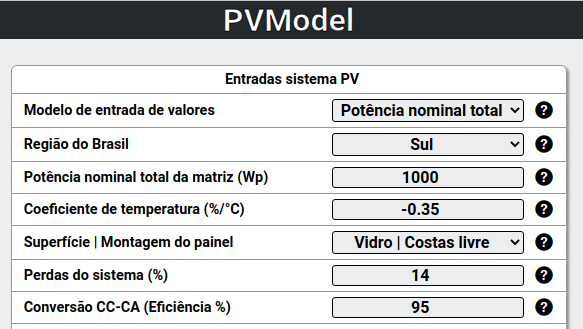
\includegraphics[width=0.95\textwidth]{./Figuras/modelo1.png}
    \caption{Entradas do sistema ``potência nominal total''}
   \label{fig:modelo1}
\end{figure}
\newpage
\textbf{Área total}

\begin{itemize}
   \item Região do Brasil (Seleção).
   \item Área total utilizada (m²).
   \item Área de um painel (m²) .
   \item Potência nominal de um painel ($W_{p}$).
   \item Quantidade painéis.
   \item Potência nominal total da matriz $W_{p}$.
   \item Coeficiente de temperatura (\%/°C).
   \item Superfície | Montagem do painel (Seleção).
   \item Perdas do sistema (\%).
   \item Conversão CC-CA (Eficiência \%).
\end{itemize}

\textbf{Aparência final no aplicativo}

\begin{figure}[H]
    \centering
    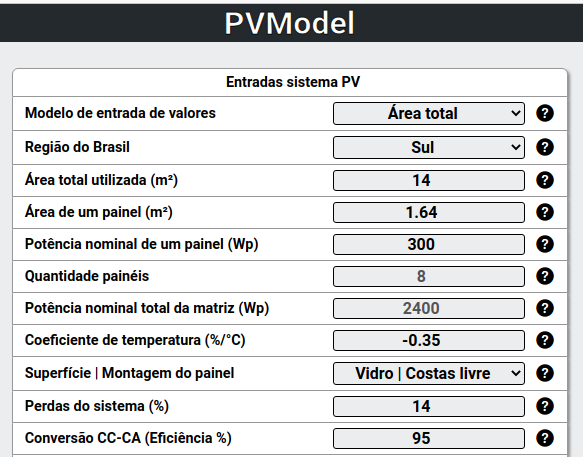
\includegraphics[width=1\textwidth]{./Figuras/modelo2.png}
    \caption{Entradas do sistema ``área total''.}
   \label{fig:modelo2}
\end{figure}

\textbf{Quantidade de painéis}

\begin{itemize}
   \item Região do Brasil (Seleção).
   \item Potência nominal de um painel $W_{p}$.
   \item Quantidade painéis (Unidade).
   \item Potência nominal total da matriz $W_{p}$.
   \item Coeficiente de temperatura (\%/°C).
   \item Superfície | Montagem do painel (Seleção).
   \item Perdas do sistema (\%).
   \item Conversão CC-CA (Eficiência \%).
\end{itemize}

\textbf{Aparência final do aplicativo}

\begin{figure}[H]
    \centering
    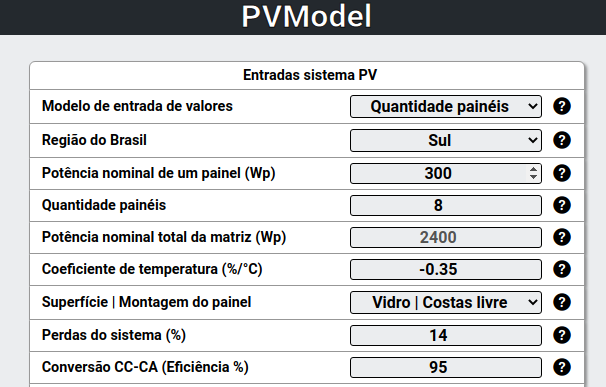
\includegraphics[width=1\textwidth]{./Figuras/modelo3.png}
    \caption{Entradas do sistema ``quantidade de painéis''.}
   \label{fig:modelo3}
\end{figure}

\newpage
\subsection{Aplicativo entradas custos e faturamentos financeiros}

Esta seção do aplicativo foi dividida em partes:

\textbf{Entradas para o ``sistema financeiro''}

\begin{itemize}
   \item Consumo de energia média mensal (kWh).
   \item Valor compra kWh da concessionária (R\$).
   \item Valor venda kWh da concessionária (R\$).
   \item Custo mínimo mensal concessionaria (R\$).
   \item Custo Wp painel (R\$).
   \item Custo Inversor ou Otimizador (R\$).
   \item Estruturas de suporte (Seleção).
   \item Quantidade estruturas de telhado (Unidade).
   \item Custo estruturas de telhado (R\$).
   \item Quantidade estruturas de garagem (Unidade).
   \item Custo estruturas de garagem (R\$).
\end{itemize}

\textbf{Aparência final do aplicativo}

\begin{figure}[H]
    \centering
    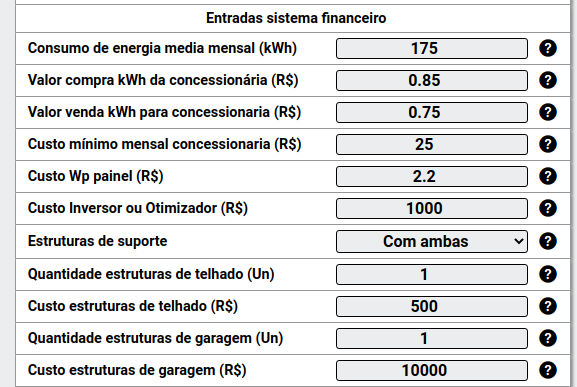
\includegraphics[width=0.9\textwidth]{./Figuras/ret_fin_1.png}
    \caption{Entradas do ``sistema financeiro''.}
   \label{fig:ret_fin_1}
\end{figure}

\newpage
\textbf{Entrada para o sistema ``estações de recarga veicular''.}

\begin{itemize}
   \item Estações de recarga VE (Seleção).
   \item Custo kWh recarga ($R\$$).
   \item Dias semana estações abertas (Unidade).
   \item Média de Horas de utilização por dia (Unidade).
\end{itemize}

\begin{figure}[H]
    \centering
    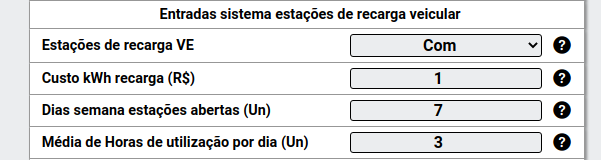
\includegraphics[width=0.875\textwidth]{./Figuras/ret_fin_2.png}
    \caption{Entradas do sistemas ``estações de recarga veicular''.}
   \label{fig:ret_fin_2}
\end{figure}

\textbf{Estações de recarga ultrarrápidas, rápidas e lenta}

\begin{itemize}
   \item Quantidade estações.
   \item Custo estações (R\$).
   \item Potência média de recarga (kW).
\end{itemize}

\begin{figure}[H]
    \centering
    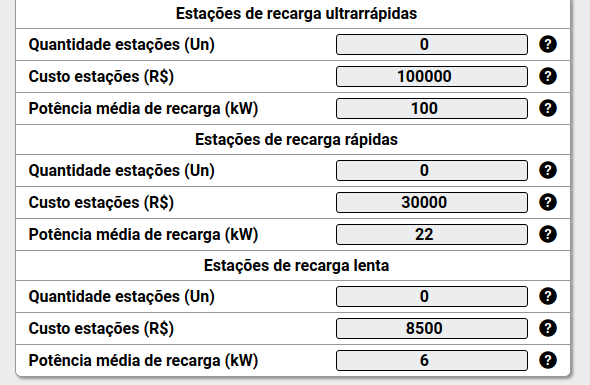
\includegraphics[width=0.9\textwidth]{./Figuras/ret_fin_3.png}
    \caption{Estações de recarga ultrarrápidas, rápidas e lenta.}
   \label{fig:ret_fin_3}
\end{figure}

\newpage

\subsection{Apresentação dos resultados}

A apresentação dos resultados foi dividida em quatro partes:

\textbf{Resultado do sistema PV ano}

\begin{itemize}
   \item Energia CA produzida total (Wh).
   \item Custo total do sistema PV (R\$).
   \item Prazo de retorno de investimento (Tempo) (Anos e meses).
\end{itemize}

\begin{figure}[H]
    \centering
    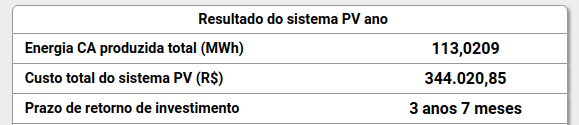
\includegraphics[width=0.85\textwidth]{./Figuras/Resultados_number_1.png}
    \caption{Resultado do sistema PV ano.}
   \label{fig:Resultados_number_1}
\end{figure}

\textbf{Resultado do sistema de estações recarga ano}

\begin{itemize}
   \item Consumo estações de recarga (Wh CA).
   \item Custo de compra de energia (Caso não produza) (R\$).
   \item Faturamento bruto (R\$).
   \item Faturamento liquido (R\$).
   \item Custo total estações (R\$).
   \item Prazo de retorno de investimento (Tempo) (Anos e meses).
\end{itemize}

\begin{figure}[H]
    \centering
    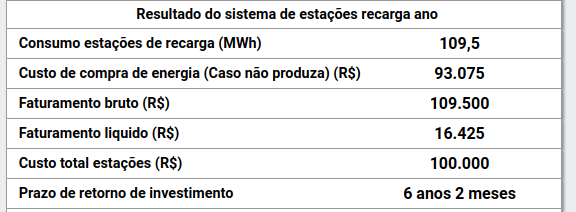
\includegraphics[width=0.85\textwidth]{./Figuras/Resultados_number_2.png}
    \caption{Resultado do sistema de estações recarga por ano.}
   \label{fig:Resultados_number_2}
\end{figure}

\newpage
\textbf{Resultado total}

\begin{itemize}
   \item Energia CA produzida total ano (Wh).
   \item Consumo total de energia ano (Wh CA).
   \item Déficit ou Excedente de energia ano (Wh CA).
   \item Valor pago ou recebido da concessionária ano (R\$).
   \item Faturamento liquido estações de recarga ano (R\$).
   \item Custo total do sistema (R\$).
   \item Prazo de retorno de investimento do sistema todo em (Tempo) (Anos e meses).
   \item Lucro anual apos sistema pago (R\$).
\end{itemize}

\begin{figure}[H]
    \centering
    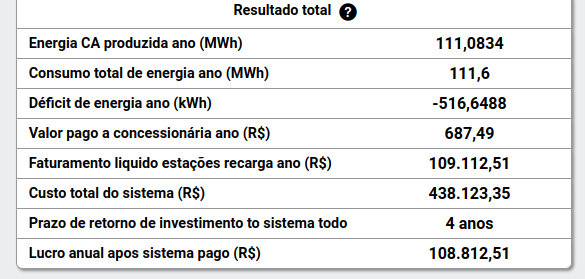
\includegraphics[width=1\textwidth]{./Figuras/Resultados_number_3.png}
    \caption{Resultado total.}
   \label{fig:Resultados_number_3}
\end{figure}

\newpage
\textbf{Resultado gráfico}

O resultado da produção de energia do sistema fotovoltaico é também apresentado graficamente por ano, mês ou dia.

\begin{figure}[H]
    \centering
    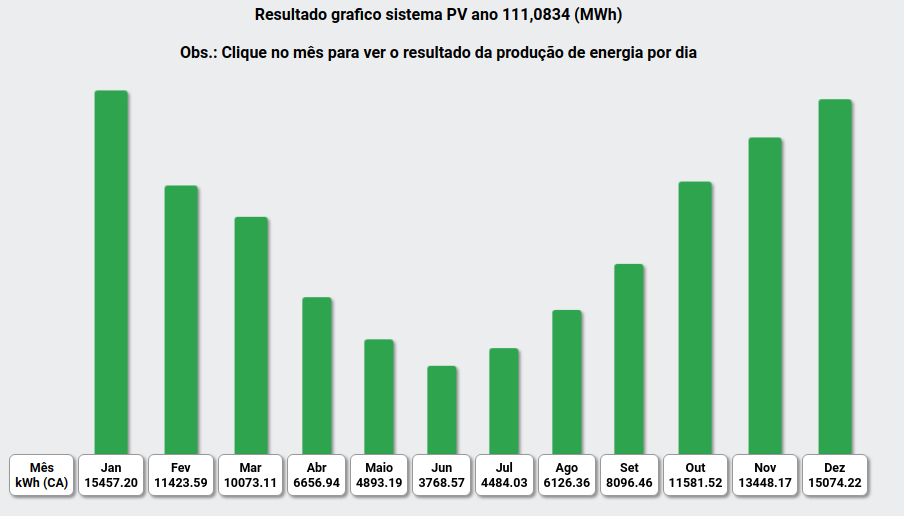
\includegraphics[width=1\textwidth]{./Figuras/modelo5.png}
    \caption{Resultados do sistema por ano.}
   \label{fig:modelo5}
\end{figure}

\begin{figure}[H]
    \centering
    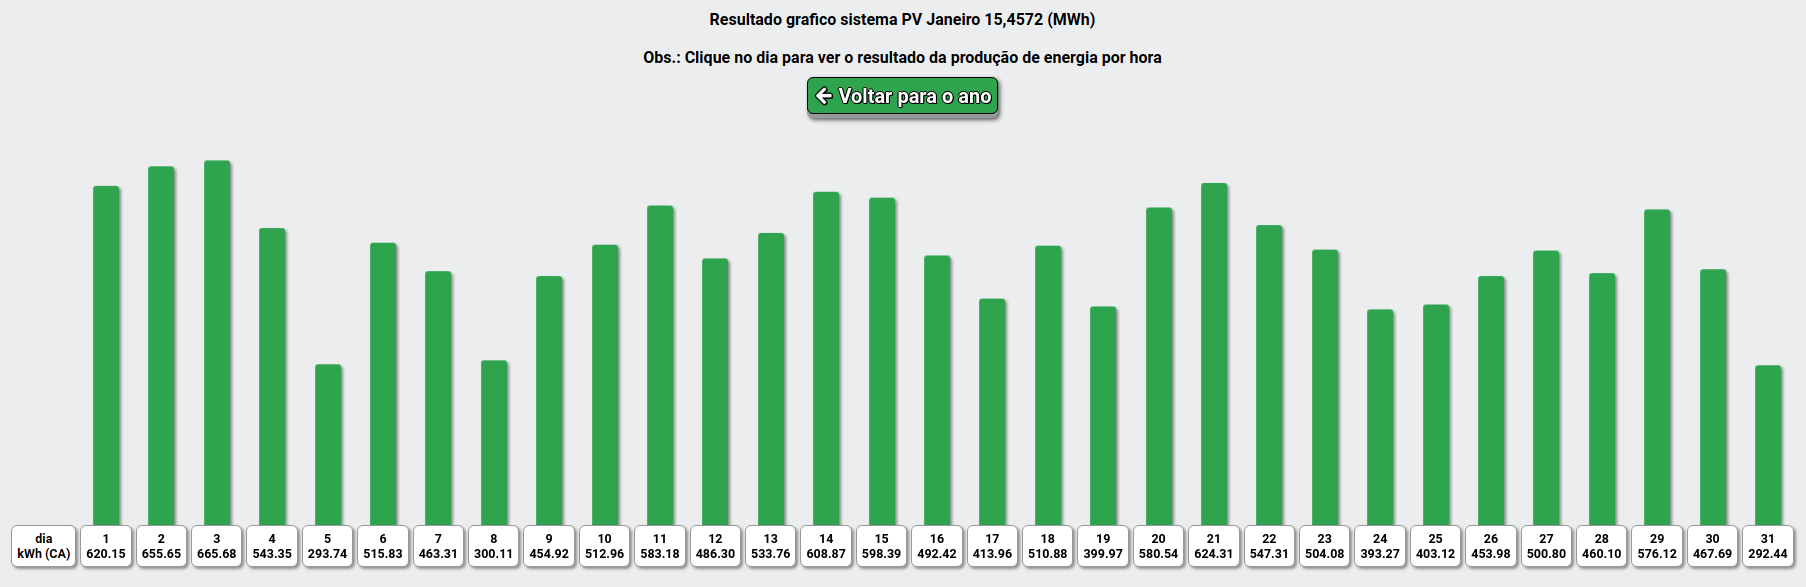
\includegraphics[width=1\textwidth]{./Figuras/modelo6.png}
    \caption{Resultados do sistema por mês.}
   \label{fig:modelo6}
\end{figure}

\begin{figure}[H]
    \centering
    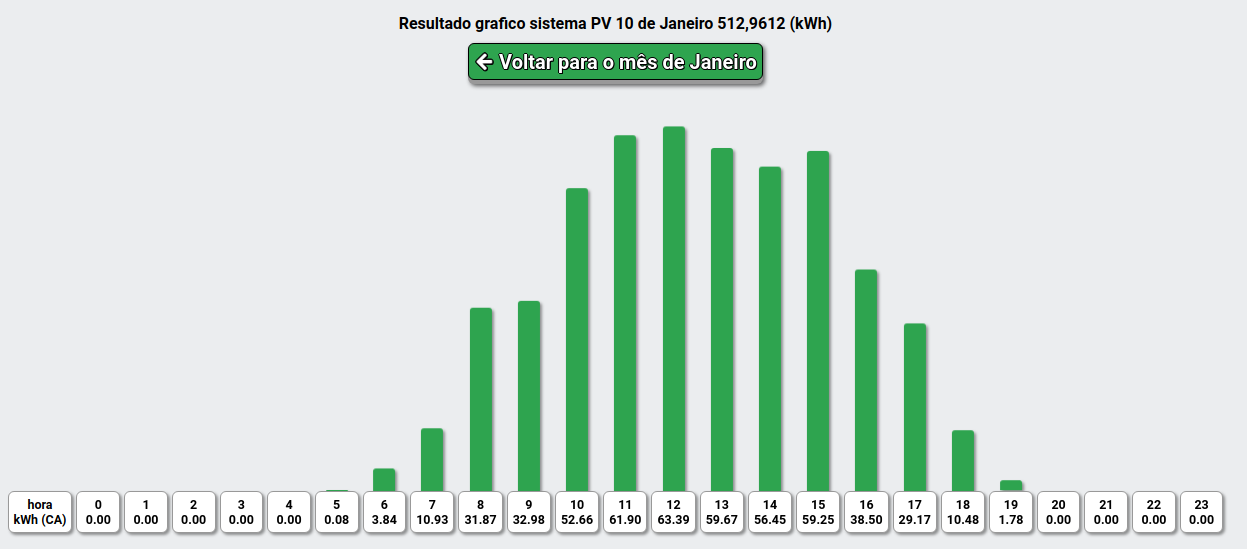
\includegraphics[width=1\textwidth]{./Figuras/modelo7.png}
    \caption{Resultados do sistema por dia.}
   \label{fig:modelo7}
\end{figure}